\documentclass[11pt,reqno]{beamer}
\usepackage[utf8]{inputenc}
\usetheme{Dresden}
\usecolortheme{beaver}
\usepackage{amsmath}
\usepackage{amsfonts}
\usepackage{graphicx}
\usepackage{stmaryrd}
\usepackage{siunitx}
\usepackage[backend=biber, style=chem-acs]{biblatex}
\setbeamertemplate{navigation symbols}{} 
\title{Bond Graph Clinic: Part 3}
\subtitle{Biomolecular Systems}
\author{Peter Cudmore}

\institute{Systems Biology Lab, The University of Melbourne}

\newcommand{\D}[2]{\frac{\mathrm{d} #1}{\mathrm{d} #2}}
\newcommand{\e}{\mathrm{e}}
\newcommand{\I}{\mathrm{i}}
\renewcommand{\mod}[1]{\left|#1\right|}
\newcommand{\DD}[2]{\frac{\mathrm{d}^2 #1}{\mathrm{d} #2^2}}
\newcommand{\bigO}[1]{\text{O}\left(#1\right)}
\renewcommand{\P}[2]{\frac{\partial #1}{\partial #2}}
\renewcommand{\Re}{\operatorname{Re}}
\renewcommand{\Im}{\operatorname{Im}}
\newcommand{\EX}{\mathbb{E}}
\newcommand{\df}[1]{\mspace{2mu}  \mathrm{d}#1}
\newcommand{\reals}{\mathbb{R}}
\newcommand{\complex}{\mathbb{C}}
\newcommand{\conj}[1]{\overline{#1}}
\bibliography{references}

\begin{document}
	\begin{frame}
	\titlepage
	\addtocounter{framenumber}{-1} 
\end{frame}
\begin{frame}
\tableofcontents[hideallsubsections]
\end{frame}
\section{Previously...}
\begin{frame}
\frametitle{Network models of energetic systems}
\begin{figure}
	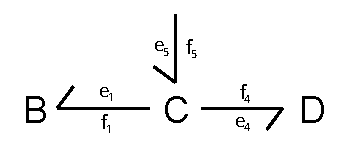
\includegraphics{images/bondgraph.pdf}
\end{figure}
Bond Graphs capture:
\begin{itemize}
	\item Energy transferred between $B,C,D$ without loss via bonds.
	\item Power transfer represented by conjugate variables $P_i=e_if_i$.
	\item Subsystem dynamics via constitutive relations $\Phi_B(e,f) = 0$
\end{itemize}
We've also looked at some examples.
\end{frame}
\begin{frame}
\frametitle{A Mathematicians Model of a Chemical System}
A naive description of molecular systems is as follows:
\begin{enumerate}
	\item A set of distinct quanta (molecules, complexes, atoms and free electrons) $A, B, \ldots$ move stochastically through a volume.
	\item When $A, B$ are sufficiently close they may bind to form complex $C$.
	\item After some time $\tau$, $C$ may disassociate into a number of quanta $E, \ldots$.
\end{enumerate}
All basic reaction types (synthesis, decomposition and replacement) can be represented in this way.\\
\vspace*{10pt}
Clearly this is an example of a \emph{reaction-diffusion} process.
\end{frame}
\begin{frame}
\frametitle{This Clinic}
Today we shall consider \emph{reactions}.
\vfill

Next clinic will consider \emph{diffusion}

\vfill

For more details to Oster, Perelson and Auslander \cite{Oster:1971aa, Oster:1971ab, Oster:1973aa, Oster:1974aa, Perelson:1974, Auslander:1972aa}
\end{frame}
\section{Chemical Reactions}
\subsection{Assumptions}
\begin{frame}
\frametitle{Spatial Assumptions}
Consider chemical reactions inside some vessel of fixed volume.\\
We assume that the chemical solution is well mixed, ie:
\begin{itemize}
	\item The solution is actively stirred or,
	\item the diffusion rate across the volume is orders of magnitude faster than the fastest reaction rate.
\end{itemize}
\vfill
This basically means we can work with average concentration, and ignore spatial effects inside the vessel.
\vfill
Later, we will couple many vessels together to represent diffusion.
\end{frame}

\begin{frame}
\frametitle{Thermodynamic Assumptions}
Consider chemical reactions inside some vessel of fixed volume.\\
We assume that the solution is \emph{isobaric} and \emph{isothermic}.
These assumptions allow us to define the chemical potential
\[
\mu_A = \mu_A^\varoslash + RT\ln \frac{x_A}{V_m}
\]
\only<1>{
\begin{itemize}
	\item $R=N_Ak_b\approx 8.314$ is the gas constant in \si{\joule\per\kelvin\per\mole}
	\item $T\approx 300$ is temperature (in \si{\kelvin})
	\item $\mu_A^\varoslash$ is the chemical potential of a pure solution of $A$ in \si{\joule}
	\item $x_A$ the amount of species $A$ in \si{\mole}.
	\item $V_m$ is volume of the solution in \si{\mole}
\end{itemize}
This follows from the \emph{Ideal Gas Law} and the \emph{Fundamental Equation of Thermodynamics}.
}
\only<2>{
\begin{eqnarray*}
\text{Energy}&=&x_A \cdot \mu_A \si{\joule} \\
\text{Power}&=&\dot{x}_A\cdot \mu_A\ \si{\joule\per\second}
\end{eqnarray*}
\begin{center}
$\mu_A$ is \emph{effort} or force-like \\
\vspace{10pt}
$\dot{x}_A$ is the \emph{flow} or flux-like.
\end{center}
\vfill
}

\only<3>{
Recall $x_A$ is the molar amount of species $A$.\\
\vfill 
Question:\\
What happens to $\mu_A$ when $x_A \rightarrow 0$ but $V_m$ is constant?\\
When might this occur and is this physical?
}
\end{frame}
\subsection{Components}
\begin{frame}
\frametitle{Ce Constitutive Relation}
\begin{figure}
	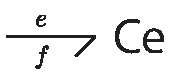
\includegraphics{images/oneport-Ce.pdf}
\end{figure}
Constitutive Relation for a Chemical Species:
\[
\Phi_A(e,f) = e - \beta \ln kq = 0 
\]
\vfill
\only<2>{
This follow from substituting the parameters 
\[
k = \exp(\mu_A^\varoslash/RT)/V_m,\qquad \beta = RT
\]
and the state variables $\mu_A = e$, $\int \mu_A\df{t} = p$, $\dot{x}_A = f$ and $x_A = q$ into 
\[
\mu_A = \mu_A^\varoslash + RT\ln \frac{x_A}{V_m}.
\]}
\only<3>{
\[
k = \exp(\mu_A^\varoslash/RT)/V_m,\qquad \beta = RT
\]
}
\end{frame}
\begin{frame}
\frametitle{Chemical Kinetics}
Reactions proceed according to the \emph{Marcelin-de Donder} formula
\[
v = \kappa\left(\e^{A^f/RT} - \e^{A^r/RT}\right)
\]
\only<1>{Here:
\begin{itemize}
	\item $v$ is the reaction velocity or molar flow
	\item $A^f, A^r$ are the forward and reverse chemical affinities
	\item $\kappa$ is the reaction rate constant.
	\item $R,T$ is the gas constant and temperature respectively.
\end{itemize}}
\only<2>{

The mass flow in is $v$, hence the mass flow out is $-v$.\\
\vspace{10pt}
So
\[
f_1 = v,\qquad f_2 = -v
\]
are natural \emph{flow} variables.

}
\only<3>{

For a chemical reaction $\nu^f_AA + \nu^f_BB +\ldots \rightleftharpoons \nu^f_AA + \nu^f_BB +\ldots$ with forward and reverse stoichiometric coefficients $\nu^f_i$ and $\nu^r_i$ for $i\in \{A,B,\ldots\}$.\\
The forward (and similarly reverse) affinity is defined as
\[
A^f = \nu^f_A\mu_A + \nu^f_B\mu_B +\ldots
\]
So the natural effort variables are
\[
e_1 =  A^f \qquad e_2 = A^r.
\]
}
\end{frame}



\end{document}